\documentclass{article}
\usepackage[utf8]{inputenc}
\usepackage[]{apacite}
\usepackage[]{graphicx}

\title{Assignment 4 - Literature draft}
\author{Ragger Jonkers - 10542604}

\begin{document}

\maketitle

\section*{Problem definition}
Take the recently leaked Panama Papers as example: how do we find interesting entities in the documents without specifically searching for a particular entity? Named Entity Recognition can extract named entities unconditionally. \\\\
Searching naively through every word in all the lobby documents per search query is slow, because most words don't provide information on what the article is about, this is especially slow with multiple query terms. If, for example, from a small document of 1000 words 10 entities were extracted that could be used for search queries, it would mean a 100 times less terms to search through. Beside the time expenditure, only exact matches will be found. For example searching for 'Wilders' will only result in documents containing 'Wilders' not also 'Geert' if 'Geert Wilders' is referred to. Entity Linking will link these concepts to their semantic representation such as their Wikipedia article.


\begin{figure}
    \centering
    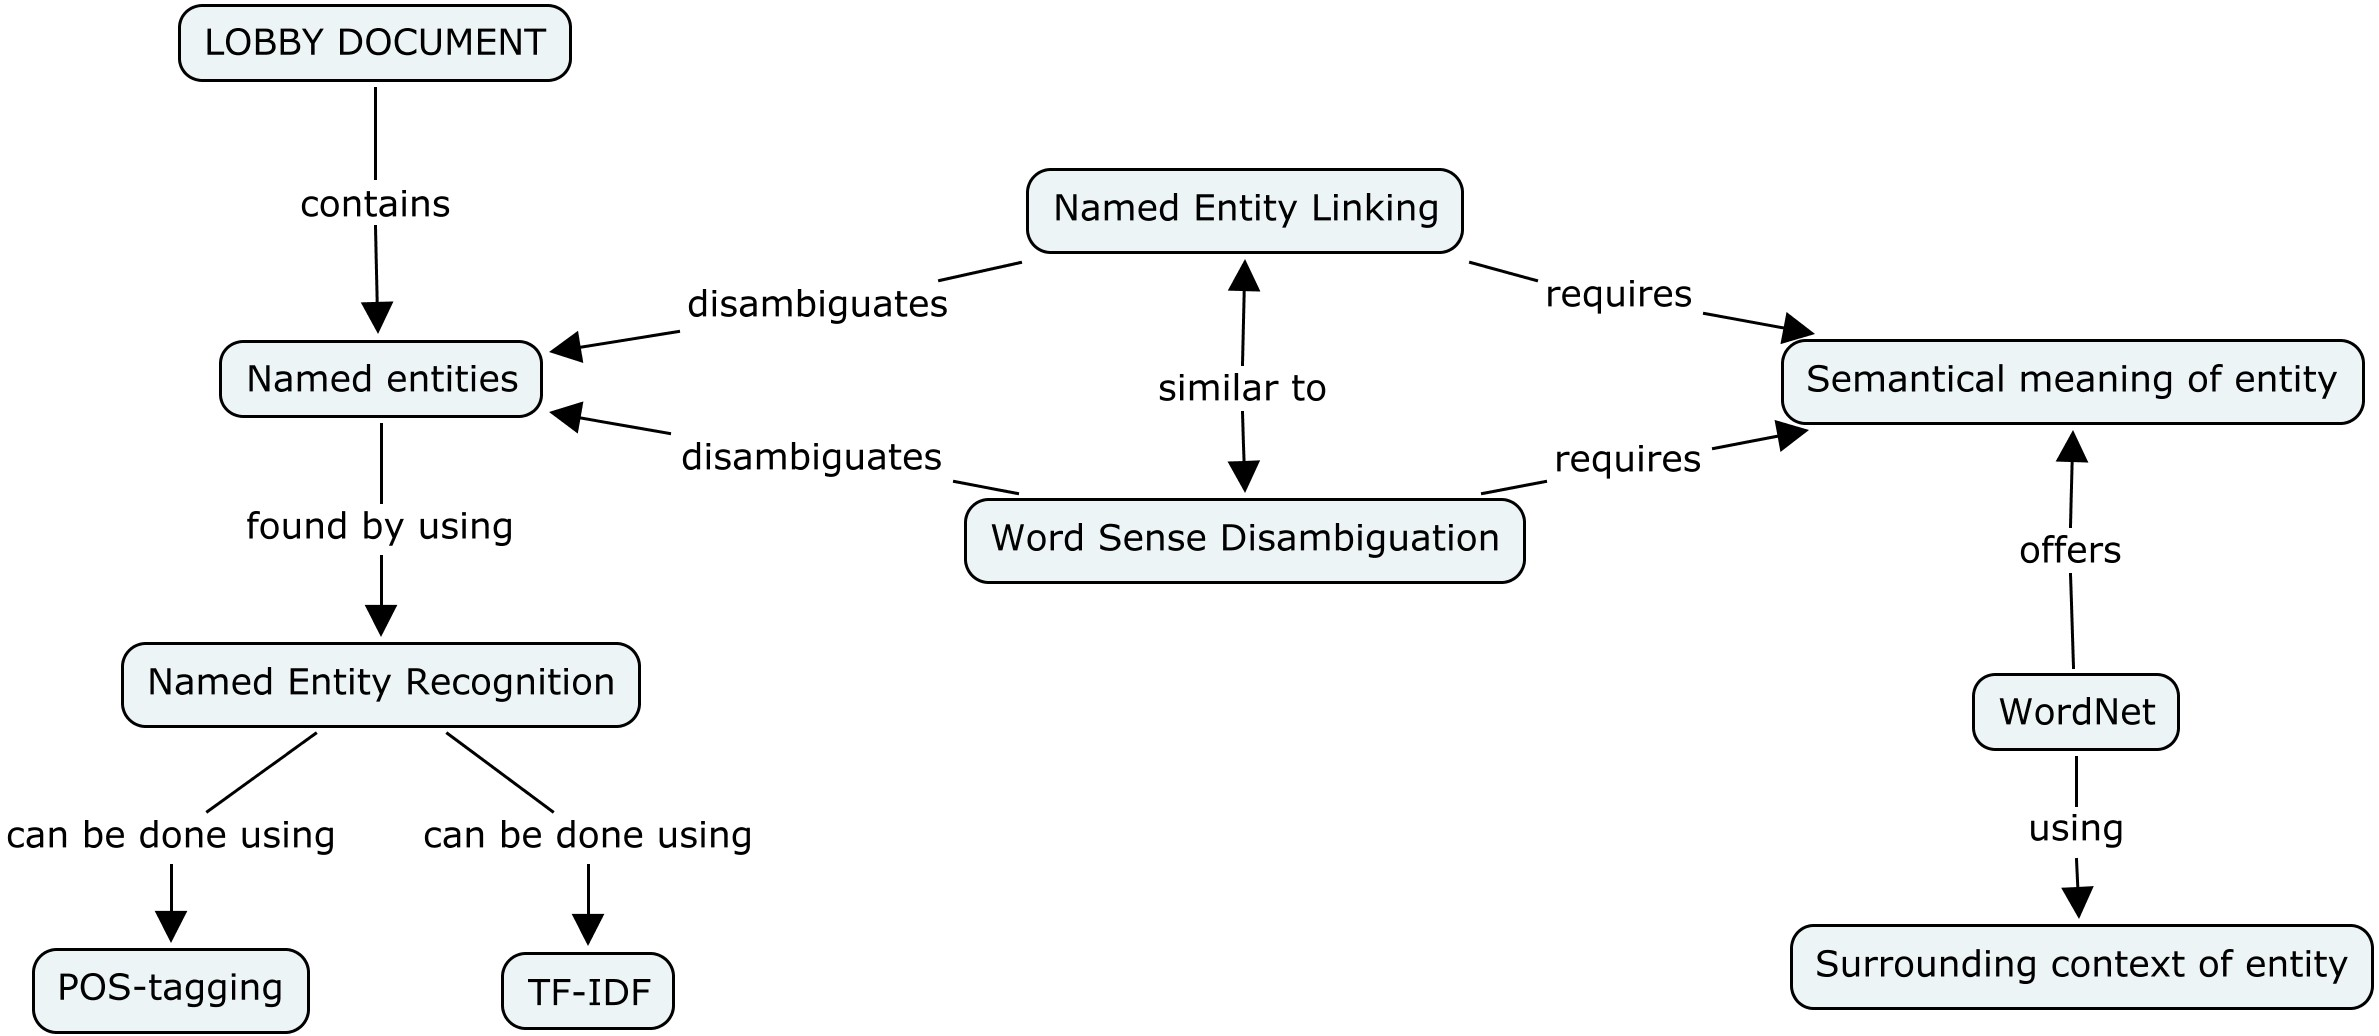
\includegraphics[scale=0.18]{Figures/ner}
    \caption{Concept map of NER}
    \label{fig:ner}
\end{figure}

\section*{Literature}
\subsection*{Graph-Based Named Entity Linking with Wikipedia}
Named entity linking (NEL) is similar to the widely-studied problem of word sense disambiguation (WSD), with Wikipedia articles playing the role of WordNet synsets \cite{hachey2011graph}. Candidate recall is not as good as literature suggests, because current disambiguaters are not performing well with a lot of candidates. A graph-based approach of NEL is competitive with today's (un)supervised approaches to NEL.

\subsection*{A Bootstrapping Approach to Named Entity Classification Using Successive Learners}
The Named Entity learner in the paper takes for each role such as PERSON, ORGANIZATION, LOCATION a set of seeds \cite{niu2003bootstrapping}. For example PERSON has seed terms as he/she/his/her/him/man/woman. If the context of the found entities have any linguistic/semantic relation to the seeds (using WordNet) that replace the entity in the sentence, then that entity must belong to that role. This approach gives the user the option to define his own roles.

\subsection*{Design Challenges and Misconceptions in Named Entity Recognition}
\textbf{External knowledge}\\
This research shows that machine learning on labeled data is not required to classify certain entities \cite{ratinov2009design}. A simple lookup in a dictionary is sufficient, called \textit{gazatteer matching}. High recall gazatteerd are used from wikipedia that cover almost all entities.\\\\
The second tool for external knowledge is word clustering on unlabeled text, known as \textit{word class models}.\\\\
\textbf{Non-local features}
Take as example “Australia” and “The bank of Australia”. The first instance should be labeled
as LOC, and the second as ORG. This can be solved using \textit{context aggregation features} (e.g. the longest capitilized sequence of words in the document which contains the current token)

\subsection*{Unsupervised named-entity extraction from the Web: An experimental study}
The KNOWITALL system aims to automate the tedious process of extracting large collections of
facts (e.g., names of scientists or politicians) from the Web in an unsupervised, domain-independent,
and scalable manner \cite{etzioni2005unsupervised}. Patterns are used in combination with phrasal structures to extract the entities.

\subsection*{Named Entity Recognition using an HMM-based Chunk Tagger}
This paper proposes a Hidden Markov Model (HMM) and an HMM-based chunk tagger, from which a named entity (NE)
recognition (NER) system is built to recognize and classify names, times and numerical quantities \cite{zhou2002named}. Given a certain token sequence, an optimal tag sequence needs to be found. A tag consists of three parts:
\begin{itemize}
    \item Boundary category (index of entity word)
    \item Category
    \item Word feature (complex)
\end{itemize}

\subsection*{Semanticizing Search Engine Queries}
The open-source \textit{Semanticizer} from the UvA is used to first generate candidate entities (known as mention detection), then disambiguate the generated entities using a binary classifier that labels entities as target entities \cite{graus2014semanticizing}. The \textit{Document ranker} assigns a higher score to entities of which the wikipedia pages are more similar to the context of the query. This way most unlikely candidates are thrown away.

\bibliography{references}
\bibliographystyle{apacite}

\end{document}